
\providecommand{\llsq}{\mathrel{\square}}%
\providecommand{\rvW}{\mathbf{W}}  %
\providecommand{\rvC}{\mathbf{C}}  %
\providecommand{\rvF}{\mathbf{F}}  %
\providecommand{\Cat}{\mathcal{C}at}%
\providecommand{\sSet}{s\mathcal{S}et}%
\providecommand{\wlim}{\operatorname{lim}}%
\providecommand{\wcolim}{\operatorname{colim}}%
\providecommand{\lan}{\operatorname{lan}}%
\providecommand{\ran}{\operatorname{ran}}%

\section{Reedy 模型结构}\label{sec:the-reedy-model-structure}

本节的目标在于说明：$\mathcal{M}$ 上的任何\trWeakFactorizationSystem{}如何
产生 $\mathcal{M}^{\mathcal{A}}$ 上的一个\emph{Reedy 弱分解系统}（Reedy weak
factorization system），进而说明：由 $\mathcal{M}$ 上一个\trModelStructure{}%
相伴的诸 Reedy 弱分解系统定义 $\mathcal{M}^{\mathcal{A}}$ 上的\emph{Reedy
\trModelStructure}。这两个结果都源自对「归纳地定义由 Reedy \trCategory{}标引
的\trFunctor{}与\trNaturalTransformation{}需要什么」所作的分析。最后，我们证
明加权\trLimit{}二函子与加权\trColimit{}二函子定义 Quillen \trBifunctor——这
是一个更一般的代数结果的重要特例——并讨论这一结果对由 Reedy \trCategory{}标引
的\trHomotopyLimit{}与\trHomotopyColimit{}理论的种种意涵。

这一工作需要一项准备：讨论上一节引入的诸骨架与诸余骨架如何在 Reedy 形状的%
\trDiagram{}的归纳定义中登场。对一个 Reedy \trCategory{} $\mathcal{A}$，记
\[
\mathcal{A}_{\le 0}\subset\mathcal{A}_{\le 1}\subset\cdots\subset
\mathcal{A}_{\le n-1}\subset\mathcal{A}_{\le n}\subset\cdots\subset\mathcal{A}
\]
为由度数至多为下标所示序数的对象组成的诸全子范畴。这些范畴为我们提供了一种
理解\cref{not:sk-cosk-diagrams}的\trSkeleton{}函子与余骨架函子的新方式。

\begin{lemma}\label{lem:kan-adjoint-triple}
对任何\trComplete{}且\trCocomplete{}的\trCategory{} $\mathcal{M}$，限制与
左、右\trKanExtension{}定义\trFunctor{}的一个\trAdjointTriple
\begin{center}
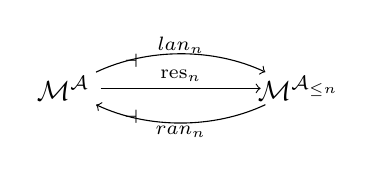
\begin{tikzpicture}[x=1.7em,y=1.4em]
  \node (M) at (0,0) {$\mathcal{M}^{\mathcal{A}}$};
  \node (Mn) at (5.0,0) {$\mathcal{M}^{\mathcal{A}_{\le n}}$};
  \draw[->] (0.7,0.42) .. controls (1.8,1.05) and (3.2,1.05) .. (4.3,0.42);
  \node at (2.5,1.12) {$\scriptstyle\lan_n$};
  \draw[->] (0.8,0) -- (4.2,0);
  \node at (2.5,0.32) {$\scriptstyle\mathrm{res}_n$};
  \node at (1.45,0.72) {$\scriptstyle\dashv$};
  \draw[->] (4.3,-0.42) .. controls (3.2,-1.05) and (1.8,-1.05) .. (0.7,-0.42);
  \node at (2.5,-1.12) {$\scriptstyle\ran_n$};
  \node at (1.45,-0.72) {$\scriptstyle\dashv$};
\end{tikzpicture}
\end{center}
其诱导的余单子 $\mathrm{sk}_n\coloneqq\lan_n\circ\mathrm{res}_n$ 与单子
$\mathrm{cosk}_n\coloneqq\ran_n\circ\mathrm{res}_n$ 相伴
$\mathrm{sk}_n\dashv\mathrm{cosk}_n$，且自然同构于由加权\trColimit{}与加权%
\trLimit{}所定义的函子
\[
\lan_n\mathrm{res}_n(-)\cong\wcolim_{\mathrm{sk}_n\mathcal{A}}-
\qquad\text{与}\qquad
\ran_n\mathrm{res}_n(-)\cong\wlim_{\mathrm{sk}_n\mathcal{A}}-.
\]
\end{lemma}
\begin{proof}
\cref{ex:prove-kan-adjoint-triple}。
\end{proof}

例如：

\begin{definition}\label{def:simplex-skeleton-coskeleton}
将上述记号特化，记 $\Delta_{\le n}\subset\Delta$ 为第 1 章中的%
\cref{not:simplex-category}的\trSimplexCategory{}中由序数
$[0],\ldots,[n]$ 张成的全子范畴。限制与左、右\trKanExtension{}定义伴随
\begin{center}
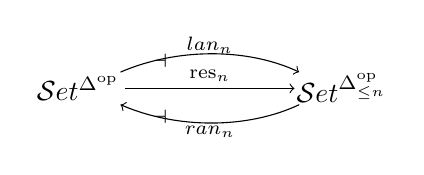
\begin{tikzpicture}[x=1.7em,y=1.4em]
  \node (S) at (0,0) {$\mathcal{S}et^{\Delta^{\mathrm{op}}}$};
  \node (T) at (5.6,0) {$\mathcal{S}et^{\Delta_{\le n}^{\mathrm{op}}}$};
  \draw[->] (0.9,0.42) .. controls (2.1,1.05) and (3.6,1.05) .. (4.7,0.42);
  \node at (2.8,1.12) {$\scriptstyle\lan_n$};
  \draw[->] (1.0,0) -- (4.6,0);
  \node at (2.8,0.32) {$\scriptstyle\mathrm{res}_n$};
  \node at (1.75,0.72) {$\scriptstyle\dashv$};
  \draw[->] (4.7,-0.42) .. controls (3.6,-1.05) and (2.1,-1.05) .. (0.9,-0.42);
  \node at (2.8,-1.12) {$\scriptstyle\ran_n$};
  \node at (1.75,-0.72) {$\scriptstyle\dashv$};
\end{tikzpicture}
\end{center}
其在 $\sSet$ 上诱导一个幂等余单子
$\mathrm{sk}_n\coloneqq\lan_n\circ\mathrm{res}_n$ 与一个幂等单子
$\mathrm{cosk}_n\coloneqq\ran_n\circ\mathrm{res}_n$，二者相伴
$\mathrm{sk}_n\dashv\mathrm{cosk}_n$。这一余单子与单子的余单位与单位定义诸%
典范映射
\[
\mathrm{sk}_n X\xrightarrow{\;\varepsilon\;}X\xrightarrow{\;\eta\;}
\mathrm{cosk}_n X
\]
把单纯集 $X$ 与其\textbf{$n$-\trSkeleton}（$n$-skeleton）及\textbf{$n$-余骨架}
（$n$-coskeleton）联系起来。若上述映射中的前者、相应地后者，是\trIsomorphism，
我们便说 $X$ 是\textbf{$n$-骨架的}（$n$-skeletal）或\textbf{$n$-余骨架的}
（$n$-coskeletal）。
\end{definition}
下述引理记录了由全忠实包含
$\mathrm{sk}_n\mathcal{A}\hookrightarrow\mathcal{A}$ 所产生的\trAdjointTriple{}
$\lan_n\dashv\mathrm{res}_n\dashv\ran_n$ 的若干特殊性质。特别地，从单纯集的
$n$-\trSkeleton{}到其 $n$-余骨架的\trCanonical{}映射可以在更一般的情形下定义，
而不只是对作为限制而定义的诸\trDiagram：

\begin{lemma}\label{lem:fully-faithful-adjoint-triple}
对任何\trFullyFaithful{}包含 $\mathcal{B}\hookrightarrow\mathcal{A}$ 与%
\trComplete{}且\trCocomplete{}的\trCategory{} $\mathcal{M}$，试考虑相伴的%
\trAdjointTriple：
\begin{center}
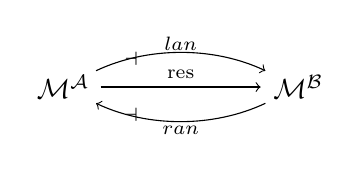
\begin{tikzpicture}[x=1.7em,y=1.4em]
  \node (M) at (0,0) {$\mathcal{M}^{\mathcal{A}}$};
  \node (Mb) at (5.0,0) {$\mathcal{M}^{\mathcal{B}}$};
  \draw[->] (0.7,0.42) .. controls (1.8,1.05) and (3.2,1.05) .. (4.3,0.42);
  \node at (2.5,1.12) {$\scriptstyle\lan$};
  \draw[->] (0.8,0) -- (4.2,0);
  \node at (2.5,0.32) {$\scriptstyle\mathrm{res}$};
  \node at (1.45,0.72) {$\scriptstyle\dashv$};
  \draw[->] (4.3,-0.42) .. controls (3.2,-1.05) and (1.8,-1.05) .. (0.7,-0.42);
  \node at (2.5,-1.12) {$\scriptstyle\ran$};
  \node at (1.45,-0.72) {$\scriptstyle\dashv$};
\end{tikzpicture}
\end{center}
\begin{enumerate}[label=(\roman*)]
\item 诸\trFunctor{} $\lan$，$\ran\colon\mathcal{M}^{\mathcal{B}}\to\mathcal{M}^{\mathcal{A}}$
  是\trFullyFaithful{}；也就是说，$\lan\dashv\mathrm{res}$ 的\trUnit{}%
  与 $\mathrm{res}\dashv\ran$ 的\trCounit{}是\trIsomorphism。
\item 下方交换方块中的公共复合定义一个\trCanonical{}\trNaturalTransformation
\begin{center}
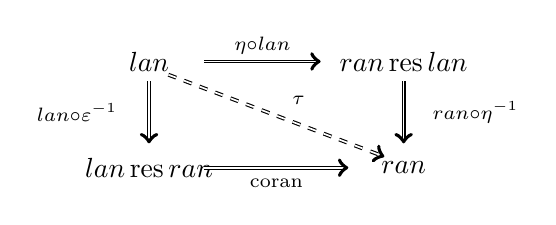
\begin{tikzpicture}[x=2.0em,y=1.6em]
  \node (lan) at (0,1.3) {$\lan$};
  \node (rrl) at (4.6,1.3) {$\ran\,\mathrm{res}\,\lan$};
  \node (lrr) at (0,-1.1) {$\lan\,\mathrm{res}\,\ran$};
  \node (ran) at (4.6,-1.1) {$\ran$};
  \draw[double,->] (1.0,1.3) -- (3.1,1.3);
  \node at (2.05,1.66) {$\scriptstyle\eta\circ\lan$};
  \draw[double,->] (0,0.85) -- (0,-0.55);
  \node at (-1.3,0.15) {$\scriptstyle\lan\circ\varepsilon^{-1}$};
  \draw[double,->] (4.6,0.85) -- (4.6,-0.55);
  \node at (5.9,0.15) {$\scriptstyle\ran\circ\eta^{-1}$};
  \draw[double,->] (1.0,-1.1) -- (3.6,-1.1);
  \node at (2.3,-1.46) {$\scriptstyle\mathrm{coran}$};
  \draw[double,dashed,->] (0.35,1.0) -- (4.25,-0.85);
  \node at (2.7,0.42) {$\scriptstyle\tau$};
\end{tikzpicture}
\end{center}
\end{enumerate}
\end{lemma}

虽然我们觉得 (ii) 中的交换方块颇为有趣，但由于包含 $\mathcal{B}\hookrightarrow\mathcal{A}$
是全忠实的，$\tau$ 其实可以更简单地定义：利用左、右\trKanExtension{}的%
\trUniversalProperty，把它取作延拓给定图表的始\trFunctor{}与终\trFunctor。

\begin{proof}
众所周知：一支\trRightAdjoint{}\trFunctor{}是\trFullyFaithful{}，当且仅当
其余单位是\trIsomorphism；而且沿全忠实\trFunctor{}的\trPointwise{}右%
\trKanExtension{}之余单位是\trIsomorphism；至于证明，请把第 9 章中的%
\cref{lem:fully-faithful-characterizations}与\cref{prop:extensions-along-fully-faithful}
的结果特化到 ∞-宇宙 $\Cat$ 之上。这些陈述及其对偶证明了 (i)。

在 (ii) 中，$\tau$ 被定义为 $\eta^{-1}\colon\mathrm{res}\,\lan\Rightarrow\mathrm{id}$
在 $\mathrm{res}\dashv\ran$ 之下的伴随转置，同时也可被定义为
$\varepsilon^{-1}\colon\mathrm{id}\Rightarrow\mathrm{res}\,\ran$ 在
$\lan\dashv\mathrm{res}$ 之下的伴随转置。为见这两个定义相符，请注意：前者
断言下方右侧两个态射的复合是左侧态射的唯一右逆，而后者断言下方左侧两个态射
的复合是右侧态射的唯一左逆：
\[
\mathrm{id}\;\underset{\cong}{\xRightarrow{\;\eta\;}}\;
\mathrm{res}\,\lan\;\xRightarrow{\;\mathrm{res}\,\tau\;}\;
\mathrm{res}\,\ran\;\underset{\cong}{\xRightarrow{\;\varepsilon\;}}\;
\mathrm{id}
\]
换言之，两个定义都恰好断言：所示的三重复合是恒同。
\end{proof}

以这种方式，我们得到一个\trNaturalTransformation{}
$\tau_n\colon\mathrm{sk}_n\Rightarrow\mathrm{cosk}_n$，它介于\cref{lem:kan-adjoint-triple}
中引入的余单子与单子之间。这些结构使我们得以归纳地定义 Reedy \trDiagram：

\begin{proposition}[图表的归纳定义]\label{prop:inductive-definition-of-diagrams}
\begin{enumerate}[label=(\roman*)]
\item 一个\trDiagram{} $X\in\mathcal{M}^{\mathcal{A}_{\le n-1}}$ 连同对
  $\mathcal{A}$ 中每个度数为 $n$ 的对象 $a$ 的一族因子分解
\begin{center}
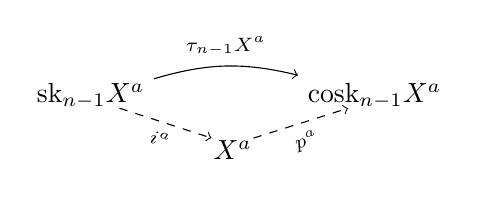
\begin{tikzpicture}[x=1.9em,y=1.5em]
  \node (sk) at (0,1.3) {$\mathrm{sk}_{n-1}X^{a}$};
  \node (ck) at (5.4,1.3) {$\mathrm{cosk}_{n-1}X^{a}$};
  \node (X) at (2.7,0) {$X^{a}$};
  \draw[->] (sk) to[bend left=15] node[above]{$\scriptstyle\tau_{n-1}X^{a}$} (ck);
  \draw[->,dashed] (0.55,1.0) -- (2.3,0.28) node[pos=0.5,below,sloped]{$\scriptstyle i^{a}$};
  \draw[->,dashed] (3.1,0.28) -- (4.9,1.0) node[pos=0.5,below,sloped]{$\scriptstyle p^{a}$};
\end{tikzpicture}
\end{center}
  唯一地确定 $X$ 到一个\trDiagram{} $X\in\mathcal{M}^{\mathcal{A}_{\le n}}$
  的扩张。
\item 一个\trNaturalTransformation{} $f\colon X\to Y\in\mathcal{M}^{\mathcal{A}_{\le n-1}}$
  连同对 $\mathcal{A}$ 中每个度数为 $n$
  的对象 $a$ 的一族因子分解
\begin{center}
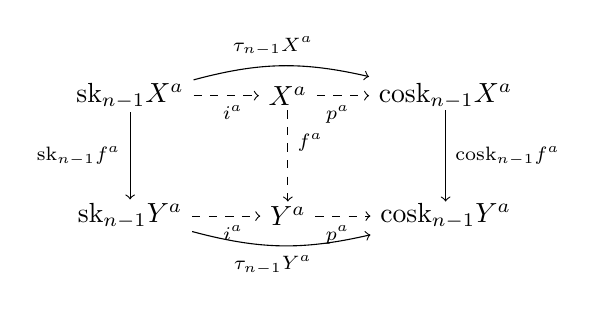
\begin{tikzpicture}[x=1.9em,y=1.5em]
  \node (skX) at (0,2.4) {$\mathrm{sk}_{n-1}X^{a}$};
  \node (XX) at (3.0,2.4) {$X^{a}$};
  \node (ckX) at (6.0,2.4) {$\mathrm{cosk}_{n-1}X^{a}$};
  \node (skY) at (0,-0.5) {$\mathrm{sk}_{n-1}Y^{a}$};
  \node (YY) at (3.0,-0.5) {$Y^{a}$};
  \node (ckY) at (6.0,-0.5) {$\mathrm{cosk}_{n-1}Y^{a}$};
  \draw[->] (skX) to[bend left=14] node[above,pos=0.45]{$\scriptstyle\tau_{n-1}X^{a}$} (ckX);
  \draw[->,dashed] (skX) -- node[below,pos=0.6]{$\scriptstyle i^{a}$} (XX);
  \draw[->,dashed] (XX) -- node[below,pos=0.4]{$\scriptstyle p^{a}$} (ckX);
  \draw[->] (0,2.0) -- (0,-0.1) node[midway,left]{$\scriptstyle\mathrm{sk}_{n-1}f^{a}$};
  \draw[->,dashed] (3.0,2.05) -- (3.0,-0.15) node[pos=0.35,right]{$\scriptstyle f^{a}$};
  \draw[->] (6.0,2.05) -- (6.0,-0.15) node[midway,right]{$\scriptstyle\mathrm{cosk}_{n-1}f^{a}$};
  \draw[->,dashed] (skY) -- node[below,pos=0.6]{$\scriptstyle i^{a}$} (YY);
  \draw[->,dashed] (YY) -- node[below,pos=0.4]{$\scriptstyle p^{a}$} (ckY);
  \draw[->] (skY) to[bend right=14] node[below,pos=0.45]{$\scriptstyle\tau_{n-1}Y^{a}$} (ckY);
\end{tikzpicture}
\end{center}
  唯一地确定 $f$ 到一个映射 $f\colon X\to Y\in\mathcal{M}^{\mathcal{A}_{\le n}}$
  的扩张。
\end{enumerate}
\end{proposition}

\begin{proof}
对于 (i)，尚待定义 $X$ 在定义域或陪域度数为 $n$ 的非恒同态射上的作用。
任何此类态射 $k\colon a\to a'$ 的 Reedy 分解经由一个度数小于 $n$ 的对象 $b$。
通过复合右上或左下方块中的映射，存在唯一的点线箭头映射使下图交换
\begin{center}
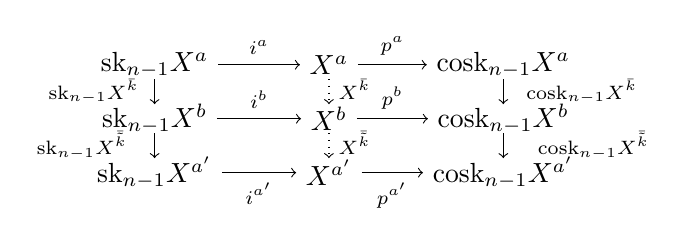
\begin{tikzpicture}[x=2.1em,y=1.5em]
  \node (a1) at (0,2.6) {$\mathrm{sk}_{n-1}X^{a}$};
  \node (a2) at (3.0,2.6) {$X^{a}$};
  \node (a3) at (6.0,2.6) {$\mathrm{cosk}_{n-1}X^{a}$};
  \node (b1) at (0,1.3) {$\mathrm{sk}_{n-1}X^{b}$};
  \node (b2) at (3.0,1.3) {$X^{b}$};
  \node (b3) at (6.0,1.3) {$\mathrm{cosk}_{n-1}X^{b}$};
  \node (c1) at (0,0) {$\mathrm{sk}_{n-1}X^{a'}$};
  \node (c2) at (3.0,0) {$X^{a'}$};
  \node (c3) at (6.0,0) {$\mathrm{cosk}_{n-1}X^{a'}$};
  \draw[->] (a1) -- node[above]{$\scriptstyle i^{a}$} (a2);
  \draw[->] (a2) -- node[above]{$\scriptstyle p^{a}$} (a3);
  \draw[->] (b1) -- node[above]{$\scriptstyle i^{b}$} (b2);
  \draw[->] (b2) -- node[above]{$\scriptstyle p^{b}$} (b3);
  \draw[->] (c1) -- node[below]{$\scriptstyle i^{a'}$} (c2);
  \draw[->] (c2) -- node[below]{$\scriptstyle p^{a'}$} (c3);
  \draw[->] (0,2.25) -- (0,1.65);
  \node at (-1.05,1.95) {$\scriptstyle\mathrm{sk}_{n-1}X^{\bar{k}}$};
  \draw[->] (0,0.95) -- (0,0.35);
  \node at (-1.25,0.65) {$\scriptstyle\mathrm{sk}_{n-1}X^{\bar{\tilde{k}}}$};
  \draw[->,dotted] (3.0,2.25) -- (3.0,1.65) node[pos=0.4,right]{$\scriptstyle X^{\bar{k}}$};
  \draw[->,dotted] (3.0,0.95) -- (3.0,0.35) node[pos=0.4,right]{$\scriptstyle X^{\bar{\tilde{k}}}$};
  \draw[->] (6.0,2.25) -- (6.0,1.65);
  \node at (7.35,1.95) {$\scriptstyle\mathrm{cosk}_{n-1}X^{\bar{k}}$};
  \draw[->] (6.0,0.95) -- (6.0,0.35);
  \node at (7.55,0.65) {$\scriptstyle\mathrm{cosk}_{n-1}X^{\bar{\tilde{k}}}$};
\end{tikzpicture}
\end{center}
而这些映射复合起来便定义了 $X$ 在 $k$ 上的作用。这一构造在可复合态射对
$k\cdot h$ 上的函子性，由\trCategory{} $\mathcal{F}act_{\le n-1}(k\cdot h)$
的连通性得出。对于 (ii)，将 (i) 应用于\trDiagram{}
$a\mapsto f^{a}\colon\mathcal{A}_{\le n-1}\to\mathcal{M}^{\mathbf{2}}$。
\end{proof}

现在我们把注意力转向本节的主旨。设 $\mathcal{M}$ 是一个配有%
\trWeakFactorizationSystem{} $(\mathrm{L},\mathrm{R})$ 的\trCategory，并设
$\mathcal{A}$ 是一个 Reedy \trCategory。

\begin{definition}\label{def:reedy-weak-factorization-system}
相对于 $\mathcal{M}$ 上的\trWeakFactorizationSystem{} $(\mathrm{L},\mathrm{R})$
而定义的 $\mathcal{M}^{\mathcal{A}}$ 上的\textbf{Reedy 弱分解系统}
$(\mathrm{L}[\mathcal{A}],\mathrm{R}[\mathcal{A}])$ 由如下组成：
\begin{itemize}
\item 左类 $\mathrm{L}[\mathcal{A}]$：那些映射 $f\colon X\to Y\in\mathcal{M}^{\mathcal{A}}$，
  其相对锁存映射（relative latching map）
  $\widehat{\ell}^{a}f\colon\ell^{a}f\to Y^{a}\in\mathcal{M}$ 落于
  $\mathrm{L}$ 中；并且
\item 右类 $\mathrm{R}[\mathcal{A}]$：那些映射 $f\colon X\to Y\in\mathcal{M}^{\mathcal{A}}$，
  其相对匹配映射 $\widehat{m}^{a}f\colon X^{a}\to m^{a}f\in\mathcal{M}$ 落于 $\mathrm{R}$ 中。
\end{itemize}
我们说一个映射 $f\colon X\to Y\in\mathcal{M}^{\mathcal{A}}$ 在 $\mathrm{L}$
中是 \textbf{Reedy} 的或在 $\mathrm{R}$ 中是 \textbf{Reedy} 的，若其相对锁存
映射或相对匹配映射分别居于 $\mathrm{L}$ 或 $\mathrm{R}$ 中。
\end{definition}

诸类 $\mathrm{L}[\mathcal{A}]$ 与 $\mathrm{R}[\mathcal{A}]$ 分别是诸类
$\mathrm{L}$ 与 $\mathrm{R}$ 沿 $\mathcal{A}$-标引的\trFunctor{}族
$\widehat{\ell}^{a}\colon(\mathcal{M}^{\mathcal{A}})^{\mathbf{2}}\to\mathcal{M}^{\mathbf{2}}$
或 $\widehat{m}^{a}\colon(\mathcal{M}^{\mathcal{A}})^{\mathbf{2}}\to\mathcal{M}^{\mathbf{2}}$ 的提升。
由函子性，我们看出这两个类对\trRetract{}封闭。现在，\cref{ex:retract-argument}
与下述一对引理相结合便蕴含：这两个类确实在\trCategory{}
$\mathcal{M}^{\mathcal{A}}$ 上定义一个\trWeakFactorizationSystem。

\begin{lemma}\label{lem:reedy-lifting}
$\mathrm{L}[\mathcal{A}]$ 中的诸映射对 $\mathrm{R}[\mathcal{A}]$ 中的诸映射
具有左\trLifting{}性质。
\begin{center}
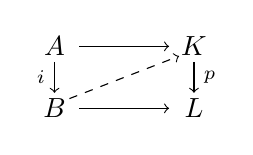
\begin{tikzpicture}[x=1.8em,y=1.6em]
  \node (A) at (0,1.4) {$A$};
  \node (K) at (2.8,1.4) {$K$};
  \node (B) at (0,0) {$B$};
  \node (L) at (2.8,0) {$L$};
  \draw[->] (0.5,1.4) -- (2.3,1.4);
  \draw[->] (0,1.05) -- (0,0.35) node[midway,left]{$\scriptstyle i$};
  \draw[->] (2.8,1.05) -- (2.8,0.35) node[midway,right]{$\scriptstyle p$};
  \draw[->] (0.5,0) -- (2.3,0);
  \draw[->,dashed] (0.3,0.22) -- (2.5,1.18);
\end{tikzpicture}
\end{center}
\end{lemma}
\begin{proof}
由\cref{lem:right-lifting-closure}与\cref{cor:morphism-cell-complex}，为证对任何态射对 $i$，
$p\in\mathcal{M}^{\mathcal{A}}$ 有 $i\llsq p$，只需求解下方左侧在
$\mathcal{M}^{\mathcal{A}}$ 中对每个 $a\in\mathcal{A}$ 的\trLifting{}问题
\begin{center}
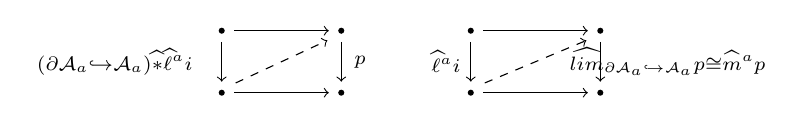
\begin{tikzpicture}[x=1.8em,y=1.6em]
  \fill (0,1.4) circle (1.1pt);
  \fill (2.4,1.4) circle (1.1pt);
  \fill (0,0) circle (1.1pt);
  \fill (2.4,0) circle (1.1pt);
  \draw[->] (0.25,1.4) -- (2.15,1.4);
  \draw[->] (0,1.15) -- (0,0.25);
  \node at (-2.15,0.7) {$\scriptstyle(\partial\mathcal{A}_a\hookrightarrow\mathcal{A}_a)\mathbin{\widehat{\ast}}\widehat{\ell}^{a} i$};
  \draw[->] (2.4,1.15) -- (2.4,0.25);
  \node at (2.78,0.7) {$\scriptstyle p$};
  \draw[->] (0.25,0) -- (2.15,0);
  \draw[->,dashed] (0.28,0.22) -- (2.12,1.18);
  \node at (3.55,0.7) {$\leftrightsquigarrow$};
  \begin{scope}[shift={(5.0,0)}]
    \fill (0,1.4) circle (1.1pt);
    \fill (2.6,1.4) circle (1.1pt);
    \fill (0,0) circle (1.1pt);
    \fill (2.6,0) circle (1.1pt);
    \draw[->] (0.25,1.4) -- (2.35,1.4);
    \draw[->] (0,1.15) -- (0,0.25);
    \node at (-0.5,0.7) {$\scriptstyle\widehat{\ell}^{a} i$};
    \draw[->] (2.6,1.15) -- (2.6,0.25);
    \node at (3.95,0.7) {$\scriptstyle\widehat{\wlim}_{\partial\mathcal{A}_a\hookrightarrow\mathcal{A}_a}p\cong\widehat{m}^{a}p$};
    \draw[->] (0.25,0) -- (2.35,0);
    \draw[->,dashed] (0.28,0.22) -- (2.32,1.18);
  \end{scope}
\end{tikzpicture}
\end{center}
经伴随，只需求解上方右侧 $\mathcal{M}$ 中的转置\trLifting{}问题（见%
\cref{lem:adjunction-transposes-lifting}）。若 $i\in\mathrm{L}[\mathcal{A}]$
且 $p\in\mathrm{R}[\mathcal{A}]$，则由定义 $\widehat{\ell}^{a}i\in\mathrm{L}$
且 $\widehat{m}^{a}p\in\mathrm{R}$，故解存在。
\end{proof}

\begin{lemma}\label{lem:reedy-factorization}
每个映射 $f\colon X\to Y\in\mathcal{M}^{\mathcal{A}}$ 都可以分解为
$\mathrm{L}[\mathcal{A}]$ 中一个映射接 $\mathrm{R}[\mathcal{A}]$ 中一个映射。
\end{lemma}

\begin{proof}
我们对 $f^{a}\colon X^{a}\to Y^{a}$ 的分解之诸分量按 $a$ 的度数归纳地定义。
一开始，我们用 $(\mathrm{L},\mathrm{R})$ 的分解去分解所有由度数为零的对象所
标引的分量。由于由这些对象张成的全子范畴 $\mathcal{A}_{\le0}$ 只有恒同箭头，
这就定义了子\trDiagram{} $f\in\mathcal{M}^{\mathcal{A}_{\le0}}$ 的一个分解。

继续归纳，假设我们已把限制 $f\in\mathcal{M}^{\mathcal{A}_{<n}}$ 分解为
\begin{center}
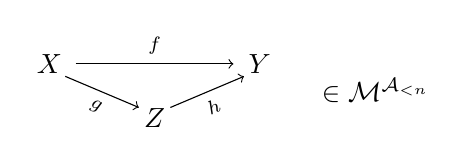
\begin{tikzpicture}[x=1.9em,y=1.5em]
  \node (X) at (0,1.3) {$X$};
  \node (Y) at (4.0,1.3) {$Y$};
  \node (Z) at (2.0,0) {$Z$};
  \draw[->] (0.5,1.3) -- (3.5,1.3) node[midway,above]{$\scriptstyle f$};
  \draw[->] (0.3,1.0) -- (1.7,0.25) node[pos=0.5,below,sloped]{$\scriptstyle g$};
  \draw[->] (2.3,0.25) -- (3.7,1.0) node[pos=0.5,below,sloped]{$\scriptstyle h$};
  \node at (6.2,0.65) {$\in\mathcal{M}^{\mathcal{A}_{<n}}$};
\end{tikzpicture}
\end{center}
其中对所有度数小于 $n$ 的对象 $a$ 有 $\widehat{\ell}^{a}g\in\mathrm{L}$ 且
$\widehat{m}^{a}h\in\mathrm{R}$。由\cref{prop:inductive-definition-of-diagrams}，
为定义随之而来的 $f^{a}$ 的分解，只需定义 $\mathcal{M}$ 中一个对象 $Z^{a}$
连同点线箭头映射。
\begin{center}
\begin{tikzpicture}[x=1.9em,y=1.5em]
  \node (LX) at (0,2.6) {$L^{a}X$};
  \node (LZ) at (3.2,2.6) {$L^{a}Z$};
  \node (LY) at (6.4,2.6) {$L^{a}Y$};
  \node (PU) at (2.1,1.8) {$\scriptstyle X^{a}\underset{L^{a}X}{\sqcup}L^{a}Z$};
  \node (Xa) at (0,1.0) {$X^{a}$};
  \node (Za) at (3.2,1.0) {$Z^{a}$};
  \node (Ya) at (6.4,1.0) {$Y^{a}$};
  \node (PB) at (4.6,0.2) {$\scriptstyle M^{a}Z\underset{M^{a}Y}{\times}Y^{a}$};
  \node (MX) at (0,-0.8) {$M^{a}X$};
  \node (MZ) at (3.2,-0.8) {$M^{a}Z$};
  \node (MY) at (6.4,-0.8) {$M^{a}Y$};
  \draw[->] (0.65,2.6) -- (2.35,2.6);
  \draw[->] (3.95,2.6) -- (5.7,2.6);
  \draw[->] (1.75,2.4) -- (PU);
  \draw[->] (0.35,1.25) -- (1.4,1.72);
  \node at (1.2,1.98) {$\scriptstyle\ulcorner$};
  \draw[->,dotted] (2.65,1.6) -- (3.0,1.22) node[pos=0.4,right]{$\scriptstyle\widehat{\ell}^{a} g$};
  \draw[->,dotted] (0.55,1.0) -- (2.5,1.0) node[midway,below]{$\scriptstyle g^{a}$};
  \draw[->,dotted] (3.9,1.0) -- (5.7,1.0) node[midway,above]{$\scriptstyle h^{a}$};
  \draw[->,dotted] (3.5,0.78) -- (4.15,0.4) node[pos=0.5,left]{$\scriptstyle\widehat{m}^{a} h$};
  \draw[->] (4.25,0.02) -- (3.55,-0.6);
  \draw[->] (5.15,0.38) -- (6.15,0.82);
  \node at (5.15,0.02) {$\scriptstyle\lrcorner$};
  \draw[->] (0,2.25) -- (0,1.35);
  \draw[->,dotted] (3.2,2.25) -- (3.2,1.35);
  \draw[->] (6.4,2.25) -- (6.4,1.35);
  \draw[->] (0,0.65) -- (0,-0.45);
  \draw[->,dotted] (3.2,0.65) -- (3.2,-0.45);
  \draw[->] (6.4,0.65) -- (6.4,-0.45);
  \draw[->] (0.65,-0.8) -- (2.5,-0.8);
  \draw[->] (3.95,-0.8) -- (5.7,-0.8);
\end{tikzpicture}
\end{center}
我们用 $(\mathrm{L},\mathrm{R})$ 分解从\trPushout{}到\trPullback{}的虚对角
映射，以定义对象 $Z^{a}$。左、右两个因子分别成为如此定义的复合态射 $g^{a}$
与 $h^{a}$ 的第 $a$ 个相对锁存映射与匹配映射。注意由构造这两个映射分别居于
类 $\mathrm{L}$ 与 $\mathrm{R}$ 中。
由\trPushout{}与\trPullback{}的\trUniversalProperty{}可得
$f^{a}=h^{a}\cdot g^{a}$。由\cref{prop:inductive-definition-of-diagrams}，
这些定义把\trNaturalTransformation{} $g$ 与 $h$ 扩张到度数 $n$。
\end{proof}

由\cref{prop:leibniz-construction-preserves}与\cref{cor:morphism-cell-complex} 可得：若
$\mathcal{M}$ 上\trWeakFactorizationSystem{} $(\mathrm{L},\mathrm{R})$ 的左类
是余纤维性生成或\trCell{}式生成的——如\cref{def:cell-complex}中那样——则
Reedy \trWeakFactorizationSystem{}的左类亦然：

\begin{proposition}\label{prop:reedy-cellularly-generated}
若 $(\mathrm{L},\mathrm{R})$ 是 $\mathcal{M}$ 上一个由映射之集 $\mathrm{J}$
\trCell{}式或余纤维性生成的\trWeakFactorizationSystem，则 $\mathcal{M}^{\mathcal{A}}$
上的 Reedy \trWeakFactorizationSystem{} $(\mathrm{L}[\mathcal{A}],\mathrm{R}[\mathcal{A}])$ 相应地由映射之集
\[
\{(\partial\mathcal{A}_a\hookrightarrow\mathcal{A}_a)\mathbin{\widehat{\ast}} j
\}_{a\in\mathcal{A},\,j\in\mathrm{J}}
\]
\trCell{}式或余纤维性地生成。
\end{proposition}

\begin{proof}
由\cref{cor:morphism-cell-complex}，任何态射 $f\colon X\to Y\in\mathcal{M}^{\mathcal{A}}$ 都可以
表示为一个由胞腔
\[
\{(\partial\mathcal{A}_a\hookrightarrow\mathcal{A}_a)\mathbin{\widehat{\ast}}
\widehat{\ell}^{a}f\}_{a\in\mathcal{A}}
\]
构筑的\trCellComplex。若 $f\in\mathrm{L}[\mathcal{A}]$，则对每个 $a$ 有
$\widehat{\ell}^{a}f\in\mathrm{L}$，且由假设，这些相对锁存映射可以表示为由
$\mathrm{J}$ 中诸映射构筑的\trCellComplex{}或\trCellComplex{}的\trRetract。
由\cref{prop:leibniz-construction-preserves}(vii)，\trLeibnizTensor{}
$(\partial\mathcal{A}_a\hookrightarrow\mathcal{A}_a)\mathbin{\widehat{\ast}}\widehat{\ell}^{a}f$ 于是可以表示为由\trBoundary{}包含与 $\mathrm{J}$ 中诸
映射的\trLeibnizTensor{}构筑的（\trRetract{}）\trCellComplex——恰如陈述中
所述。
\end{proof}

例如，单纯集的诸\trMonomorphism{}由单纯形\trBoundary{}包含
$\partial\Delta[n]\hookrightarrow\Delta[n]$（$n\ge 0$）\trCell{}式生成。

\begin{lemma}\label{lem:mono-epi-reedy-sset}
定义于 $\sSet=\mathcal{S}et^{\Delta^{\mathrm{op}}}$ 上、相对于
$\mathcal{S}et$ 上的（\trMonomorphism，\trEpimorphism）
\trWeakFactorizationSystem{}而言的 Reedy \trWeakFactorizationSystem{}
$(\mathrm{mono}[\Delta^{\mathrm{op}}],\mathrm{epi}[\Delta^{\mathrm{op}}])$，
与（\trMonomorphism，\trTrivialFibration）\trWeakFactorizationSystem{}相重合。
由此，单纯集的任何\trMonomorphism{}都\trCanonical{}地分解为诸映射
$\partial\Delta[n]\hookrightarrow\Delta[n]$（$n\ge 0$）之余积的\trPushout{}%
的序列复合。
\end{lemma}

\begin{proof}
集合的诸\trMonomorphism{}由单个映射——包含 $!\colon\varnothing\hookrightarrow\ast$——\trCell{}式生成。于是，由\cref{prop:reedy-cellularly-generated}，Reedy
\trWeakFactorizationSystem{}也是\trCell{}式生成的。在此情形，推出积函子
$-\mathbin{\widehat{\ast}}!\colon\mathcal{S}et^{\Delta^{\mathrm{op}}}\to\mathcal{S}et^{\Delta^{\mathrm{op}}}$ 是恒等，故生成映射之集即我们所熟知的
单纯形\trBoundary{}包含 $\{\partial\Delta[n]\hookrightarrow\Delta[n]\}_{n\in\Delta}$——
平凡纤维化恰由对它们的右\trLifting{}性质来刻画（见第 1 章中的%
\cref{def:trivial-fibration}）。
\end{proof}

\begin{proposition}\label{prop:reedy-components}
\begin{enumerate}[label=(\roman*)]
\item 若 $f\colon X\to Y\in\mathcal{M}^{\mathcal{A}}$ 在 $\mathrm{L}$ 中是
  Reedy 的——也就是说，若诸相对锁存映射 $\widehat{\ell}^{a}f$ 落于
  $\mathrm{L}$ 中——则每个分量 $f^{a}\colon X^{a}\to Y^{a}$ 与每支\trLatchingMap
  $L^{a}f\colon L^{a}X\to L^{a}Y$ 也落于 $\mathrm{L}$ 中。
\item 若 $f\colon X\to Y\in\mathcal{M}^{\mathcal{A}}$ 在 $\mathrm{R}$ 中是
  Reedy 的——也就是说，若诸相对匹配映射 $\widehat{m}^{a}f$ 落于
  $\mathrm{R}$ 中——则每个分量 $f^{a}\colon X^{a}\to Y^{a}$ 与每支匹配映射
  $M^{a}f\colon M^{a}X\to M^{a}Y$ 也落于 $\mathrm{R}$ 中。
\end{enumerate}
\end{proposition}

\begin{proof}
映射 $f^{a}$ 与 $L^{a}f$ 分别是 $f$ 带映射 $\varnothing\hookrightarrow\mathcal{A}^{a}$
与 $\varnothing\hookrightarrow\partial\mathcal{A}^{a}$ 的
Leibniz 加权\trColimit。把\cref{thm:canonical-cell-complex} 的\trCellComplex{}表示的协变变量在
$a\in\mathcal{A}$ 处求值，我们看出 $\varnothing\hookrightarrow\mathcal{A}^{a}$
是一个\trCellComplex，其\trCell{}具有形式
\begin{rveq}\label{eq:cell-boundary-inclusion}
\bigl((\partial\mathcal{A}_x)^{a}\hookrightarrow\mathcal{A}_{x}^{a}\bigr)
\mathbin{\widehat{\square}}
\bigl(\partial\mathcal{A}^{x}\hookrightarrow\mathcal{A}^{x}\bigr),
\end{rveq}
由诸对象 $x\in\mathcal{A}$ 标引。事实上，只需考虑那些满足
$\mathrm{deg}(x)\le\mathrm{deg}(a)$ 的对象，因为当
$\mathrm{deg}(x)>\mathrm{deg}(a)$ 时，包含 $(\partial\mathcal{A}_x)^{a}\hookrightarrow\mathcal{A}_{x}^{a}$——从而\trCell{}
\eqref{eq:cell-boundary-inclusion}——是\trIsomorphism。类似地，由于
$\partial\mathcal{A}^{a}=\mathrm{sk}_{\mathrm{deg}(a)-1}\mathcal{A}^{a}$，
\cref{thm:canonical-cell-complex} 蕴含：$\varnothing\hookrightarrow\partial\mathcal{A}^{a}$ 是一个%
\trCellComplex，其\trCell{}具有形式 \eqref{eq:cell-boundary-inclusion} 且
满足 $\mathrm{deg}(x)<\mathrm{deg}(a)$。

由\cref{prop:leibniz-construction-preserves}(vii)，映射 $f^{a}$ 与 $L^{a}f$
于是都是由\trCell{}构筑的\trCellComplex，这些\trCell{}由满足
$\mathrm{deg}(x)\le\mathrm{deg}(a)$ 与相应地 $\mathrm{deg}(x)<\mathrm{deg}(a)$
的对象 $x\in\mathcal{A}$ 标引，且具有形式
\begin{rveq}\label{eq:leibniz-cell-latching}
\widehat{\wcolim}_{\bigl((\partial\mathcal{A}_x)^{a}\hookrightarrow
\mathcal{A}_{x}^{a}\bigr)\mathbin{\widehat{\square}}
\bigl(\partial\mathcal{A}^{x}\hookrightarrow\mathcal{A}^{x}\bigr)}f
\cong\bigl((\partial\mathcal{A}_x)^{a}\hookrightarrow\mathcal{A}_{x}^{a}\bigr)
\mathbin{\widehat{\ast}}\widehat{\ell}^{x}f,
\end{rveq}
其中的\trIsomorphism{}来自\cref{prop:leibniz-construction-preserves}(i)。由
\cref{lem:set-tensor-leibniz}，\trMonomorphism{}与\trWeakFactorizationSystem{}%
左类中一个映射的\trLeibnizTensor{}仍在左类中。于是，由于
$(\partial\mathcal{A}_x)^{a}\hookrightarrow\mathcal{A}_{x}^{a}$ 是%
\trMonomorphism{}且 $\widehat{\ell}^{x}f$ 落于 $\mathrm{L}$ 中，这些%
\trCell——从而映射 $f^{a}$ 与 $L^{a}f$——也落于 $\mathrm{L}$ 中。
\end{proof}

回忆\cref{def:model-structure}：\trCategory{} $\mathcal{M}$ 上带有满足%
\trTwoOfThreeProperty{}的\trWeakEquivalence{}类 $\rvW$ 的\trModelStructure{}%
由映射的两个类 $\rvC$ 与 $\rvF$ 给出，使得 $(\rvC\cap\rvW,\rvF)$ 与
$(\rvC,\rvF\cap\rvW)$ 定义\trWeakFactorizationSystem。为证相对于
$\mathcal{M}$ 上一个\trModelStructure{}而言的诸 Reedy
\trWeakFactorizationSystem{}在 $\mathcal{M}^{\mathcal{A}}$ 上以逐点定义的%
\trWeakEquivalence{}定义一个\trModelStructure，还差一条引理。

\begin{lemma}\label{lem:reedy-cw-pointwise-we}
设诸类 $(\rvW,\rvC,\rvF)$ 在 $\mathcal{M}$ 上定义一个\trModelStructure。那么
一个映射 $f\colon X\to Y\in\mathcal{M}^{\mathcal{A}}$
\begin{enumerate}[label=(\roman*)]
\item 在 $\rvC\cap\rvW$ 中是 Reedy 的，当且仅当 $f$ 在 $\rvC$ 中是 Reedy 的
  且是\trPointwise{}\trWeakEquivalence；并且
\item 在 $\rvF\cap\rvW$ 中是 Reedy 的，当且仅当 $f$ 在 $\rvF$ 中是 Reedy 的
  且是\trPointwise{}\trWeakEquivalence。
\end{enumerate}
\end{lemma}

\begin{proof}
我们证明这对对偶陈述中的第一条。若 $f$ 在 $\rvC\cap\rvW$ 中是 Reedy 的，则
显然它在 $\rvC$ 中是 Reedy 的，而\cref{prop:reedy-components}蕴含其分量
$f^{a}$ 也居于 $\rvC\cap\rvW$ 中。于是 $f$ 是\trPointwise{}\trWeakEquivalence。

对于逆命题，我们利用图
\begin{center}
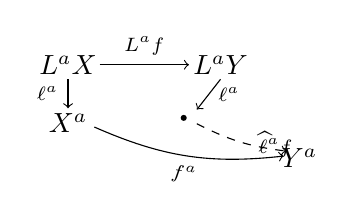
\begin{tikzpicture}[x=1.9em,y=1.5em]
  \node (LX) at (0,2.0) {$L^{a}X$};
  \node (LY) at (2.9,2.0) {$L^{a}Y$};
  \node (Xa) at (0,0.6) {$X^{a}$};
  \fill (2.2,0.72) circle (1.1pt);
  \node (Ya) at (4.4,-0.25) {$Y^{a}$};
  \draw[->] (0.6,2.0) -- (2.3,2.0) node[midway,above]{$\scriptstyle L^{a}f$};
  \draw[->] (0,1.65) -- (0,0.95) node[midway,left]{$\scriptstyle\ell^{a}$};
  \draw[->] (2.9,1.65) -- (2.45,0.92) node[pos=0.5,right]{$\scriptstyle\ell^{a}$};
  \node at (1.4,1.02) {$\scriptstyle\lrcorner$};
  \draw[->] (0.5,0.5) to[bend right=15] node[pos=0.5,below,sloped]{$\scriptstyle f^{a}$} (4.1,-0.2);
  \draw[->,dashed] (2.45,0.58) to[bend right=10] node[pos=0.6,right]{$\scriptstyle\widehat{\ell}^{a} f$} (4.15,-0.08);
\end{tikzpicture}
\end{center}
它把映射 $L^{a}f$、$\widehat{\ell}^{a}f$ 与 $f^{a}$ 对任何 $a\in\mathcal{A}$
联系起来；这是\cref{prop:leibniz-construction-preserves}(vi) 应用于
$(\varnothing\hookrightarrow\partial\mathcal{A}^{a}\hookrightarrow\mathcal{A}^{a})\mathbin{\widehat{\ast}}_{\mathcal{A}}f$ 的一个实例。假设 $f$
在 $\rvC$ 中是 Reedy 的且是\trPointwise{}\trWeakEquivalence。由%
\cref{prop:reedy-components}，可得 $L^{a}f$ 落于 $\rvC$ 中。我们将证明
$L^{a}f$ 事实上落于 $\rvC\cap\rvW$ 中，然后应用\trWeakFactorizationSystem{}%
左类的\trPushout{}稳定性与\trTwoOfThreeProperty，得出
$\widehat{\ell}^{a}f\in\rvW$，从而 $f$ 在 $\rvC\cap\rvW$ 中是 Reedy 的。我们
作归纳论证。若 $a$ 的度数为零，则 $L^{a}f$ 是\trInitial{}对象处的恒同，当然
是一个\trWeakEquivalence，而 $\widehat{\ell}^{a}f=f^{a}$ 落于 $\rvC\cap\rvW$
中。若 $a$ 的度数为 $n$，则我们现在可以假定：对任何度数小于 $a$ 之度数的 $x$
有 $\widehat{\ell}^{x}f\in\rvC\cap\rvW$。由\cref{prop:reedy-components}的
证明，$L^{a}f$ 可以表示为一个\trCellComplex，其\trCell{}
\eqref{eq:leibniz-cell-latching} 是\trMonomorphism{}与落于 $\rvC\cap\rvW$ 中
的映射的\trLeibnizTensor，因而居于 $\rvC\cap\rvW$ 中。于是我们得出
$L^{a}f\in\rvC\cap\rvW$，证明完毕。
\end{proof}

\cref{lem:reedy-lifting}、\cref{lem:reedy-factorization}与
\cref{lem:reedy-cw-pointwise-we} 合起来证明：

\begin{theorem}[Reedy 模型结构]\label{thm:reedy-model-structure}
若 $\mathcal{A}$ 是一个 Reedy \trCategory{}且 $(\rvW,\rvC,\rvF)$ 在
$\mathcal{M}$ 上定义一个\trModelStructure，则诸 Reedy
\trWeakFactorizationSystem{} $(\rvC\cap\rvW[\mathcal{A}],\rvF[\mathcal{A}])$
与 $(\rvC[\mathcal{A}],\rvF\cap\rvW[\mathcal{A}])$ 在 $\mathcal{M}^{\mathcal{A}}$
上以\trPointwise{}\trWeakEquivalence{}定义一个\trModelStructure。
\end{theorem}

Reedy \trModelStructure{}之所以重要的一个原因在于：它配备了以下列方式产生的
便利的 Quillen \trBifunctor。

\begin{theorem}\label{thm:functor-tensor-product-leibniz}
设 $\mathcal{A}$ 是一个 Reedy \trCategory，并设 $\otimes\colon\mathcal{V}\times\mathcal{M}\to\mathcal{N}$
是一个相对于\trWeakFactorizationSystem{} $(\mathrm{L},\mathrm{R})$、$(\mathrm{L}',\mathrm{R}')$
与 $(\mathrm{L}'',\mathrm{R}'')$ 的左 Leibniz \trBifunctor。
那么\trFunctor{}张量积
\[
\otimes_{\mathcal{A}}\colon\mathcal{V}^{\mathcal{A}^{\mathrm{op}}}\times
\mathcal{M}^{\mathcal{A}}\to\mathcal{N}
\]
相对于 $(\mathrm{L}'',\mathrm{R}'')$ 与 Reedy \trWeakFactorizationSystem{}
$(\mathrm{L}[\mathcal{A}^{\mathrm{op}}],\mathrm{R}[\mathcal{A}^{\mathrm{op}}])$
与 $(\mathrm{L}'[\mathcal{A}],\mathrm{R}'[\mathcal{A}])$ 是左 Leibniz 的。
\end{theorem}
$F\in\mathcal{V}^{\mathcal{A}^{\mathrm{op}}}$ 与 $G\in\mathcal{M}^{\mathcal{A}}$
的\textbf{\trFunctor{}\trTensorProduct}由余端（coend）定义
\[
F\otimes_{\mathcal{A}}G\coloneqq\int\limits^{a\in\mathcal{A}}Fa\otimes Ga
\coloneqq\mathrm{coeq}\left(\;
\coprod_{a,b\in\mathcal{A}}\mathcal{A}(a,b)\otimes Fa\otimes Gb
\Longrightarrow
\coprod_{a\in\mathcal{A}}Fa\otimes Ga\;\right).
\]

\begin{proof}
作为一个由余连续\trFunctor{}与\trColimit{}构筑起来的构造，\trFunctor{}张量积
在两个变量中都余连续。我们论证 $\otimes_{\mathcal{A}}$ 具有 Leibniz 性质。
\cref{cor:morphism-cell-complex} 断言：$\mathcal{V}^{\mathcal{A}^{\mathrm{op}}}$ 中的映射 $f$ 可以
构筑为\trCellComplex，其\trCell{}是\trLeibnizProduct
\[
(\partial\mathcal{A}^{a}\hookrightarrow\mathcal{A}^{a})\mathbin{\widehat{\ast}}
\widehat{\ell}_{a}f,
\]
而 $\mathcal{M}^{\mathcal{A}}$ 中的映射 $g$ 可以构筑为\trCellComplex，其%
\trCell{}是\trLeibnizProduct
\[
(\partial\mathcal{A}_b\hookrightarrow\mathcal{A}_b)\mathbin{\widehat{\ast}}
\widehat{\ell}^{b}g.
\]
由\cref{prop:leibniz-construction-preserves}(vii)，$f\widehat{\otimes}_{\mathcal{A}}g$
于是是一个\trCellComplex，其\trCell{}具有形式
\[
\bigl((\partial\mathcal{A}^{a}\hookrightarrow\mathcal{A}^{a})\mathbin{\widehat{\ast}}
\widehat{\ell}_{a}f\bigr)\widehat{\otimes}_{\mathcal{A}}
\bigl((\partial\mathcal{A}_b\hookrightarrow\mathcal{A}_b)\mathbin{\widehat{\ast}}
\widehat{\ell}^{b}g\bigr)
\cong(\partial\mathcal{A}^{a}\hookrightarrow\mathcal{A}^{a})
\mathbin{\widehat{\times}}_{\mathcal{A}}(\partial\mathcal{A}_b\hookrightarrow
\mathcal{A}_b)\mathbin{\widehat{\ast}}(\widehat{\ell}_{a}f\widehat{\otimes}
\widehat{\ell}^{b}g)
\]
说 $f$ 在 $\mathrm{L}$ 中是 Reedy 的而 $g$ 在 $\mathrm{L}'$ 中是 Reedy 的，
意味着 $\widehat{\ell}_{a}f\in\mathrm{L}$ 且 $\widehat{\ell}^{b}g\in\mathrm{L}'$。
由于 $\otimes$ 是左 Leibniz 的，由此得出
$\widehat{\ell}_{a}f\widehat{\otimes}\widehat{\ell}^{b}g\in\mathrm{L}''$。
$\mathcal{S}et^{\mathcal{A}^{\mathrm{op}}}$ 中的映射与 $\mathcal{S}et^{\mathcal{A}}$
中的映射的 Leibniz \trFunctor{}\trTensorProduct
\[
(\partial\mathcal{A}^{b}\hookrightarrow\mathcal{A}^{b})
\mathbin{\widehat{\times}}_{\mathcal{A}}(\partial\mathcal{A}_a
\hookrightarrow\mathcal{A}_a)
\]
等同于：把由那些经过一个度数严格小于 $a$ 或严格小于 $b$ 的对象的、从 $b$ 到
$a$ 的态射所组成的子集，包含入 hom-集 $\mathcal{A}^{a}_{b}=\mathcal{A}(b,a)$
之中；特别地，这一映射是\trMonomorphism。现在，把\cref{lem:set-tensor-leibniz}
应用于 $\mathcal{N}$ 上的\trWeakFactorizationSystem{}
$(\mathrm{L}'',\mathrm{R}'')$ 便可证明：这一\trMonomorphism{}与
$\widehat{\ell}_{a}f\widehat{\otimes}\widehat{\ell}^{b}g$ 的%
\trLeibnizTensor{}仍居于 $\mathrm{L}''$ 中，证明完毕。
\end{proof}
例如，由附录 A 中的\eqref{eq:functor-tensor-product}，加权\trColimit{}二函子
是由\cref{lem:set-tensor-leibniz}的集合张量二函子所定义的\trFunctor{}张量积。
把\cref{thm:functor-tensor-product-leibniz}应用于取（\trMonomorphism，
\trEpimorphism）为 $\mathcal{S}et$ 上默认的\trWeakFactorizationSystem，我们
得出：

\begin{corollary}\label{cor:weighted-functors-leibniz}
对任何\trComplete{}且\trCocomplete{}、配有\trWeakFactorizationSystem{}
$(\mathrm{L},\mathrm{R})$ 的\trCategory{} $\mathcal{M}$ 与任何 Reedy
\trCategory，加权\trColimit{}与加权\trLimit
\[
\wcolim_{-}\colon\mathcal{S}et^{\mathcal{A}}\times
\mathcal{M}^{\mathcal{A}^{\mathrm{op}}}\to\mathcal{M}
\qquad\text{与}\qquad
\wlim_{-}\colon(\mathcal{S}et^{\mathcal{A}})^{\mathrm{op}}\times
\mathcal{M}^{\mathcal{A}}\to\mathcal{M}
\]
相对于诸 Reedy \trWeakFactorizationSystem{}分别定义左、右 Leibniz \trBifunctor。
\end{corollary}

在模型范畴的设定中——笛卡尔封闭的模型范畴，或 $\mathcal{V}$-模型范畴（通过
取 $\mathcal{V}$ 为配有\cref{ex:set-model-category}之\trModelStructure{}的
$\mathcal{S}et$、或取 $\mathcal{V}$ 为该模型范畴自身，前两种情形被涵摄于其
中）——\cref{cor:weighted-functors-leibniz}特化为下述结果，它帮助我们理解
Reedy 形状\trDiagram{}的\trHomotopyLimit{}与\trHomotopyColimit。

\begin{corollary}\label{cor:reedy-quillen-weighted-functors}
设 $\mathcal{M}$ 是一个 $\mathcal{V}$-模型范畴，并设 $\mathcal{A}$ 是一个
Reedy \trCategory。那么，对 $\mathcal{V}^{\mathcal{A}}$ 中任何 Reedy
\trCofibrant{}的权 $W$，\footnote{在 $\mathcal{V}=\mathcal{S}et$ 的情形，
「Reedy 余纤维性的」应读作「Reedy 单态的」（Reedy monomorphic）。}加权\trColimit{}与加权%
\trLimit{}\trFunctor
\[
\wcolim_{W}-\colon\mathcal{M}^{\mathcal{A}^{\mathrm{op}}}\to\mathcal{M}
\qquad\text{与}\qquad
\wlim_{W}-\colon\mathcal{M}^{\mathcal{A}}\to\mathcal{M}
\]
相应地是相对于 $\mathcal{M}^{\mathcal{A}}$ 上的 Reedy
\trModelStructure{}而言的左、右 Quillen \trFunctor。
\end{corollary}
\begin{proof}
由\cref{ex:quillen-bifunctor-component}，把一个\trCofibrant{}对象代入适当的
变量时，诸 Quillen \trBifunctor{}便产生 Quillen \trFunctor。
\end{proof}

\begin{example}[同伦极限与同伦余极限]\label{exa:homotopy-limits-colimits}
取 $\mathcal{S}et^{\mathcal{A}}$ 中的终权 $1$，加权\trLimit{}便约化为通常的%
\trLimit{}\trFunctor。\trFunctor{} $1\in\mathcal{S}et^{\mathcal{A}}$ 是 Reedy
单态的，恰在对每个 $a\in\mathcal{A}$，权 $\partial\mathcal{A}^{a}$ 的元素
范畴（category of elements）为空或连通时。这成立当且仅当 $\mathcal{A}$ 具有
\textbf{余纤维性常数}（cofibrant constants），意即：任何\trModelCategory{}%
中\trCofibrant{}对象处的常值 $\mathcal{A}$-标引\trDiagram{}是 Reedy
\trCofibrant{}的。于是，我们得出：若 $\mathcal{A}$ 具有余纤维性常数，则%
\trLimit{}\trFunctor{} $\wlim\colon\mathcal{M}^{\mathcal{A}}\to\mathcal{M}$
是右 Quillen 的。
对偶地，\trColimit{}\trFunctor{} $\wcolim\colon\mathcal{M}^{\mathcal{A}}\to\mathcal{M}$
是加权\trColimit{}\trFunctor{}的特例，其权为
$\mathcal{S}et^{\mathcal{A}^{\mathrm{op}}}$ 中的终权 $1$。这一权是 Reedy
单态的，恰在诸权 $\partial\mathcal{A}_a$ 的元素范畴为空或连通时，而这成立
当且仅当 $\mathcal{A}$ 具有\textbf{纤维性常数}（fibrant constants），意即：
任何\trModelCategory{}中\trFibrant{}对象处的常值 $\mathcal{A}$-标引%
\trDiagram{}是 Reedy \trFibrant{}的。于是，我们得出：若 $\mathcal{A}$ 具有
纤维性常数，则\trColimit{}\trFunctor{} $\wcolim\colon\mathcal{M}^{\mathcal{A}}\to\mathcal{M}$
是左 Quillen 的（更多讨论见 \cite[\S9]{bib107}）。
\end{example}

在预层范畴（presheaf category）中，余纤维化常常就是诸\trMonomorphism，而稍
加一番气力，我们便可以为\cref{cor:reedy-quillen-weighted-functors}的应用辨认
出 Reedy 单态的权。例如，任何双单纯集（bisimplicial set）作为
$\sSet^{\Delta^{\mathrm{op}}}$ 中的对象都是 Reedy \trCofibrant{}的（见
\cite[14.3.7]{bib103}）。依据下述引理，Reedy 单态的\trCosimplicialObject{}%
也可以被辨认出来。

\begin{lemma}\label{lem:unaugmentable-cosimplicial}
\begin{enumerate}[label=(\roman*)]
\item 设 $X\colon\Delta\to\mathcal{S}et^{\mathcal{J}^{\mathrm{op}}}$ 是一个
  预层范畴中的\trCosimplicialObject。若 $X$ 是\emph{不可增广的}
（unaugmentable），意即余面映射对 $\delta^{0},\delta^{1}\colon X^{0}\to X^{1}$
的\trEqualizer{}为空，则 $X$ 的诸\trLatchingMap{}都是\trMonomorphism。
\item 若 $X$ 是一个预层范畴的切片\trCategory{}中不可增广的%
  \trCosimplicialObject，则 $X$ 的诸\trLatchingMap{}都是\trMonomorphism。
\end{enumerate}
\end{lemma}

\begin{proof}
由于诸锁存对象是按 $\mathcal{S}et^{\mathcal{J}^{\mathrm{op}}}$ 中某些在
$\mathcal{S}et$ 中\trPointwise{}计算的\trColimit{}定义的，我们可以把这一结果
约化到余单纯集 $X\colon\Delta\to\mathcal{S}et$ 的相应结果。余单纯集中的一个%
\trSimplex{}是「非退化的」，如果它不在某个来自 $\Delta$ 的\trMonomorphism{}%
的像中。第 $n$ 支\trLatchingMap{} $L^{n}X\to X^{n}$ 是\trMonomorphism，恰在把一个
$n$-\trSimplex{} $x$ 表示为一个非退化\trSimplex{} $z$ 在\trMonomorphism{}
$\sigma\colon[k]\rightarrowtail[n]$ 之下的像的每种表示都是唯一时。

于是假设我们有两个这样的表示 $x=\sigma\cdot z=\sigma'\cdot z'$。$\Delta$ 中
任何\trMonomorphism{} $\sigma$ 都有左逆 $\tau$，于是我们看到
$z=\tau\sigma'\cdot z'$。映射 $\tau\sigma'$ 可以分解为一个\trEpimorphism{}%
接一个\trMonomorphism。由于 $z$ 是非退化的，这一\trMonomorphism{}必是恒同，
故 $\tau\sigma'$ 是\trEpimorphism。对 $\sigma'$ 的一个左逆 $\tau'$ 重复这一
论证，我们看到 $\tau'\sigma$ 是\trEpimorphism，于是 $z$ 与 $z'$ 有相同的
度数，且两个\trEpimorphism{}都是恒同。这证明了 $z=z'$。

如果 $\Delta$ 中一个\trMonomorphism{}的诸左逆之集唯一刻画该%
\trMonomorphism，那么我们便可以断定 $\sigma$ 与 $\sigma'$ 必相等，从而这类
分解将是完全唯一的。这对 $\Delta$ 中几乎所有\trMonomorphism{}都成立，唯一的
例外是面映射 $\delta^{0},\delta^{1}\colon[0]\rightrightarrows[1]$。然而，
已假设 $X$ 是不可增广的，故不存在满足 $\delta^{0}\cdot z=\delta^{1}\cdot z$
的 $z\in X^{0}$，\footnote{原书于此印作 $z\in Z^{0}$；按等化子条件施于
$X^{0}$ 之文义，疑为 $z\in X^{0}$ 之误，此处径改。——译者注}于是
$L^{n}X\to X^{n}$ 对一切 $n$ 都是\trMonomorphism。这证明了第一条陈述。
对于第二条陈述，我们只需考虑预层 $A\in\mathcal{S}et^{\mathcal{J}^{\mathrm{op}}}$
之下的切片\trCategory{} $\mathcal{A}\backslash\mathcal{S}et^{\mathcal{J}^{\mathrm{op}}}$，
因为切片\trCategory{} $\mathcal{S}et^{\mathcal{J}^{\mathrm{op}}}_{/A}$ 等价于
$A$ 的元素范畴上的预层范畴，故此情形已为 (i) 所覆盖。\trForgetfulFunctor{}
$\mathcal{A}\backslash\mathcal{S}et^{\mathcal{J}^{\mathrm{op}}}\to\mathcal{S}et^{\mathcal{J}^{\mathrm{op}}}$
创造诸\trMonomorphism{}与连通%
\trColimit，这告诉我们：$\mathcal{A}\backslash\mathcal{S}et^{\mathcal{J}^{\mathrm{op}}}$
中\trCosimplicialObject{}\footnote{原书于此印作「complicial object」；按
(ii) 之语境（切片预层范畴上的余单纯对象），疑为「cosimplicial object」之误，
此处径改。——译者注}$X$ 的诸\trLatchingMap{} $L^{n}X\to X^{n}$ 对一切 $n>1$ 都在
$\mathcal{S}et^{\mathcal{J}^{\mathrm{op}}}$ 中计算。上文给出的直接计算证明
这些映射是\trMonomorphism，故只需再考虑 $n=0$ 与 $n=1$ 的情形。若 $X$ 是不
可增广的，则由假设，$\mathcal{S}et^{\mathcal{J}^{\mathrm{op}}}$ 中映射对
$\delta^{0},\delta^{1}\colon X^{0}\to X^{1}$ 的\trEqualizer{}是 $A$。于是，
第 0 支\trLatchingMap{} $A\to X^{0}$ 是一个等化子，从而必是\trMonomorphism。最后，
我们断言第 1 支\trLatchingMap{} $(\delta^{0},\delta^{1})\colon L^{1}X\cong X^{0}+X^{0}\to X^{1}$
是\trMonomorphism：在 $\mathcal{S}et^{\mathcal{J}^{\mathrm{op}}}$
中进而最终在 $\mathcal{S}et$ 中论证，容易看出这一映射沿其自身的\trPullback{}%
是 $A$。这就完成了「$X$ 为 Reedy 单态射」的证明。
\end{proof}

\begin{example}[几何实现与全化]\label{exa:geometric-realization-totalization}
由\cref{lem:unaugmentable-cosimplicial}，\trYonedaEmbedding{}定义一个 Reedy
\trCofibrant{}的权 $\Delta\in\sSet^{\Delta}$。加权\trColimit{}与加权%
\trLimit{}\trFunctor
\[
\wcolim_{\Delta}-\colon\mathcal{M}^{\Delta^{\mathrm{op}}}\to\mathcal{M}
\qquad\text{与}\qquad
\wlim_{\Delta}-\colon\mathcal{M}^{\Delta}\to\mathcal{M}
\]
通常以 \textbf{\trGeometricRealization} 与 \textbf{\trTotalization} 之名为
人所知。\cref{cor:reedy-quillen-weighted-functors}证明：若 $\mathcal{M}$
是一个单纯模型范畴，则这两个\trFunctor{}是左、右 Quillen 的。
\end{example}

\subsection*{练习}

\begin{exercise}\label{ex:prove-kan-adjoint-triple}
证明\cref{lem:kan-adjoint-triple}。
\end{exercise}

\begin{exercise}\label{ex:relative-unaugmentable}
（\cite[14.3.8]{bib103}）证明\cref{lem:unaugmentable-cosimplicial}的相对类比：
若 $X$ 与 $Y$ 都是预层范畴中的不可增广\trCosimplicialObject，则任何%
\trPointwise{}\trMonomorphism{} $X\to Y$ 也是 Reedy 单态射（Reedy
monomorphism），也就是说，其相对锁存映射均为单态射。
\end{exercise}











